\documentclass[a4paper]{article}
\usepackage[pdftex]{hyperref}
\usepackage[latin1]{inputenc}
\usepackage[english]{babel}
\usepackage{a4wide}
\usepackage{amsmath}
\usepackage{amssymb}
\usepackage{algorithmic}
\usepackage{algorithm}
\usepackage{ifthen}
\usepackage{listings}
\usepackage{array}
\usepackage{tabu}
% move the asterisk at the right position
\lstset{basicstyle=\ttfamily,tabsize=4,literate={*}{${}^*{}$}1}
%\lstset{language=C,basicstyle=\ttfamily}
\usepackage{moreverb}
\usepackage{palatino}
\usepackage{multicol}
\usepackage{tabularx}
\usepackage{comment}
\usepackage{verbatim}
\usepackage{color}
\usepackage{graphicx}
\usepackage{array,mathtools}
\usepackage{amsmath}
\usepackage{enumitem,amssymb}
\usepackage{pifont}
\newlist{todolist}{itemize}{2}
\setlist[todolist]{label=$\square$}
\newcommand{\cmark}{\ding{51}}%
\newcommand{\xmark}{\ding{55}}%
\newcommand{\done}{\rlap{$\square$}{\raisebox{2pt}{\large\hspace{1pt}\cmark}}%
\hspace{-2.5pt}}
\newcommand{\wontfix}{\rlap{$\square$}{\large\hspace{1pt}\xmark}}



%% pdflatex?
\newif\ifpdf
\ifx\pdfoutput\undefined
\pdffalse % we are not running PDFLaTeX
\else
\pdfoutput=1 % we are running PDFLaTeX
\pdftrue
\fi
\ifpdf
\fi
\ifpdf
\DeclareGraphicsExtensions{.pdf, .jpg}
\else
\DeclareGraphicsExtensions{.eps, .jpg}
\fi

\parindent=0cm
\parskip=0cm

\setlength{\columnseprule}{0.4pt}
\addtolength{\columnsep}{2pt}

\addtolength{\textheight}{5.5cm}
\addtolength{\topmargin}{-26mm}
\pagestyle{empty}

%%
%% Sheet setup
%% 
\newcommand{\coursename}{Computer Architecture and Programming Languages}
\newcommand{\courseno}{CO20-320241}
\newcommand*{\carry}[1][1]{\overset{#1}}
\newcolumntype{B}[1]{r*{#1}{@{\,}r}}
 
\newcommand{\sheettitle}{Homework}
\newcommand{\mytitle}{}
\newcommand{\mytoday}{{9th of December}, 2019}

% Current Assignment number
\newcounter{assignmentno}
\setcounter{assignmentno}{12}

% Current Problem number, should always start at 1
\newcounter{problemno}
\setcounter{problemno}{1}

%%
%% problem and bonus environment
%%
\newcounter{probcalc}
\newcommand{\problem}[2]{
  \pagebreak[2]
  \setcounter{probcalc}{#2}
  ~\\
  {\large \textbf{Problem \textcolor{blue}{\arabic{assignmentno}}.\textcolor{blue}{\arabic{problemno}}} \hspace{0.2cm}\textit{#1}} \refstepcounter{problemno}\vspace{2pt}\\}

\newcommand{\bonus}[2]{
  \pagebreak[2]
  \setcounter{probcalc}{#2}
  ~\\
  {\large \textbf{Bonus Problem \textcolor{blue}{\arabic{assignmentno}}.\textcolor{blue}{\arabic{problemno}}} \hspace{0.2cm}\textit{#1}} \refstepcounter{problemno}\vspace{2pt}\\}

%% some counters  
\newcommand{\assignment}{\arabic{assignmentno}}

%% solution  
\newcommand{\solution}{\pagebreak[2]{\bf Solution:}\\}

%% Hyperref Setup
\hypersetup{pdftitle={Homework \assignment},
  pdfsubject={\coursename},
  pdfauthor={},
  pdfcreator={},
  pdfkeywords={Computer Architecture and Programming Languages},
  %  pdfpagemode={FullScreen},
  %colorlinks=true,
  %bookmarks=true,
  %hyperindex=true,
  bookmarksopen=false,
  bookmarksnumbered=true,
  breaklinks=true,
  %urlcolor=darkblue
  urlbordercolor={0 0 0.7}
}

\begin{document}


\coursename \hfill Course: \courseno\\
Jacobs University Bremen \hfill \mytoday\\
Fjolla Dedaj\hfill
\vspace*{0.3cm}\\
\begin{center}
{\Large \sheettitle{} \textcolor{blue}{\assignment}\\}
\end{center}
\problem{}{0}
\solution
\\
Classification of programming languages by generation:\\
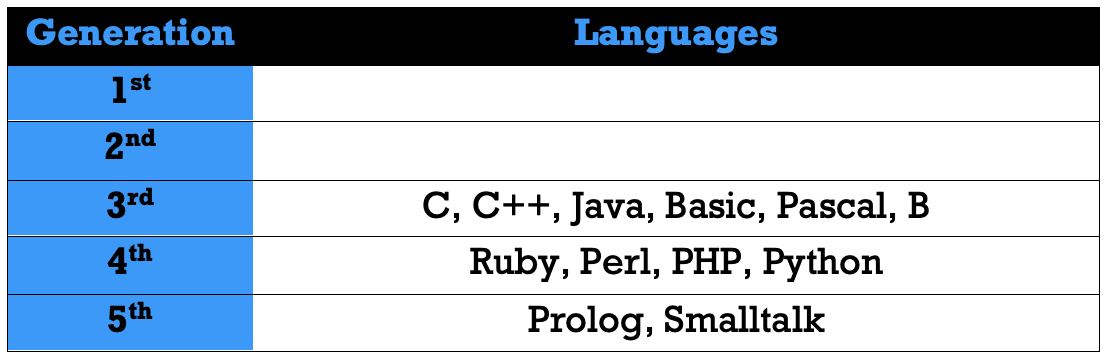
\includegraphics[scale=0.28]{1.png}\\
\\
Classification of programming languages by type:\\
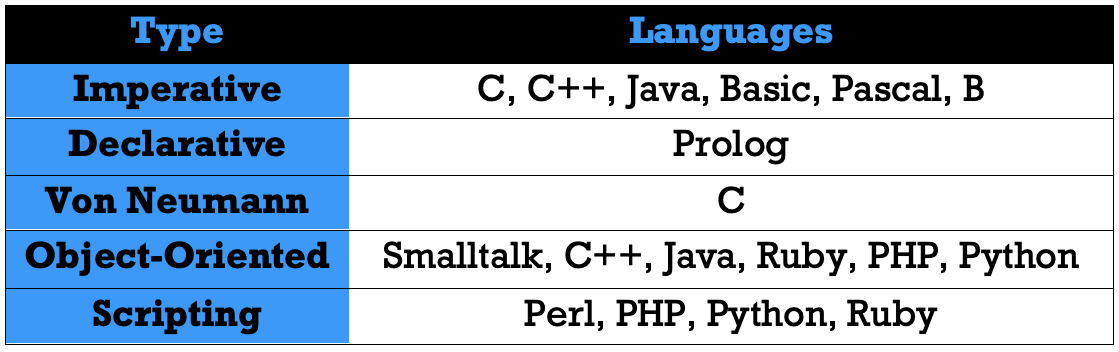
\includegraphics[scale=0.28]{2.png}
\\

\problem{}{0}
\solution
\\
trenary $\rightarrow$ var = condition ? expr1 : expr2;\\
    condition $\rightarrow$ true $|$ false $|$ var $|$ relation \\
    relation $\rightarrow$ var rel var\\
    rel $\rightarrow$ $<$ $|$ $<=$ $|$ $>$ $|$ $>=$ $|$ $==$ $|$ $!=$ \\
    expr1 $\rightarrow$ expr\\
    expr2 $\rightarrow$ expr\\
    expr $\rightarrow$ var $|$ operation\\
    operation $\rightarrow$ var op var\\
    op $\rightarrow +|-|*|/$\\
    \\
Terminals: $T=\{var, +, *, -, /, <, <=, >, >=, ==, !=, =, ?, :, ;, true, false\}$.\\
Variables of the grammar: $V=\{trenary, condition, expr1, expr2, expr, relation, operation, rel, op\}$.\\

\problem{}{0}
\solution
\\
whileloop $\rightarrow$ while(condition)\{statements\}\\
condition $\rightarrow$ identifier\text{ }rel\text{ }identifier|identifier\text{ }rel\text{ }constant\\
rel $\rightarrow$ $<|>|<=|>=|==|!=$\\
statements $\rightarrow$ statement;\text{ }statements|statement;\\
statement $\rightarrow$ var=expr\\
expr $\rightarrow$ var $|$ operation\\
operation $\rightarrow$ var\text{ }op\text{ }var\\
op $\rightarrow$ $+|-|*|/$\\
\\
Terminals: $T=\{while, (, ), \{, \}, ;, var, <, >, <=, >=, ==, !=, =, +, -, *, /\}$\\
Variables: $V=\{whileloop, condition, statements, statement, identifier, constant, rel, expr, operation, op\}$\\

\end{document}